%%%%%%%%%%%%%%%%%%%%%%%%%%%%%%%%%%%%%%%%%
% Beamer Presentation
% LaTeX Template
% Version 1.0 (10/11/12)
%
% This template has been downloaded from:
% http://www.LaTeXTemplates.com
%
% License:
% CC BY-NC-SA 3.0 (http://creativecommons.org/licenses/by-nc-sa/3.0/)
%
%%%%%%%%%%%%%%%%%%%%%%%%%%%%%%%%%%%%%%%%%

%----------------------------------------------------------------------------------------
%	PACKAGES AND THEMES
%----------------------------------------------------------------------------------------

\documentclass[handout]{beamer}

\mode<presentation> {

% The Beamer class comes with a number of default slide themes
% which change the colors and layouts of slides. Below this is a list
% of all the themes, uncomment each in turn to see what they look like.

%\usetheme{default}
%\usetheme{AnnArbor}
%\usetheme{Antibes}
%\usetheme{Bergen}
%\usetheme{Berkeley}
%\usetheme{Berlin}
%\usetheme{Boadilla}
%\usetheme{CambridgeUS}
%\usetheme{Copenhagen}
%\usetheme{Darmstadt}
%\usetheme{Dresden}
%\usetheme{Frankfurt}
%\usetheme{Goettingen}
%\usetheme{Hannover}
%\usetheme{Ilmenau}
%\usetheme{JuanLesPins}
%\usetheme{Luebeck}
\usetheme{Madrid}
%\usetheme{Malmoe}
%\usetheme{Marburg}
%\usetheme{Montpellier}
%\usetheme{PaloAlto}
%\usetheme{Pittsburgh}
%\usetheme{Rochester}
%\usetheme{Singapore}
%\usetheme{Szeged}
%\usetheme{Warsaw}

% As well as themes, the Beamer class has a number of color themes
% for any slide theme. Uncomment each of these in turn to see how it
% changes the colors of your current slide theme.

%\usecolortheme{albatross}
%\usecolortheme{beaver}
%\usecolortheme{beetle}
%\usecolortheme{crane}
%\usecolortheme{dolphin}
%\usecolortheme{dove}
%\usecolortheme{fly}
%\usecolortheme{lily}
%\usecolortheme{orchid}
%\usecolortheme{rose}
%\usecolortheme{seagull}
%\usecolortheme{seahorse}
%\usecolortheme{whale}
%\usecolortheme{wolverine}

%\setbeamertemplate{footline} % To remove the footer line in all slides uncomment this line
%\setbeamertemplate{footline}[page number] % To replace the footer line in all slides with a simple slide count uncomment this line

%\setbeamertemplate{navigation symbols}{} % To remove the navigation symbols from the bottom of all slides uncomment this line
}

\usepackage{graphicx} % Allows including images
\usepackage{booktabs} % Allows the use of \toprule, \midrule and \bottomrule in tables
\usepackage{cool}
\usepackage{amsmath}


%----------------------------------------------------------------------------------------
%	TITLE PAGE
%----------------------------------------------------------------------------------------

\title[Shelf Inventory Control]{Store-Shelf Inventory Control} % The short title appears at the bottom of every slide, the full title is only on the title page

\author{Ashwin Rao} % Your name
\institute[Stanford] % Your institution as it will appear on the bottom of every slide, may be shorthand to save space
{
ICME, Stanford University
}

\date{\today} % Date, can be changed to a custom date

\begin{document}
\begin{frame}
\titlepage % Print the title page as the first slide
\end{frame}


\begin{frame}
\frametitle{Overview}
\pause
\begin{itemize}[<+->]
\item This is a presentation on a model for inventory control that is practical
\item For real-world retail where customers browse \& shop from shelves
\item Shelf capacity and shelf emptiness are important factors
\item Customers care about ``shelf fullness'' and it influences sales
\item ``Textbook'' models of inventory control are not suitable
\item Those models essentially trade ``Holding Cost''  v/s ``Stockout Cost''
\item We develop notions of ``OverCapacity Cost'' \& ``UnderCapacity Cost''
\item Our Inventory control will essentially trade between these two costs
\item Other costs: Ordering/Moving/Labor, Spoilage \& Obsolescence 
\item Other Inputs: Demand Forecast, Shelf capacity, Casepack, Lead Time
\item Above inputs solved elsewhere as Prediction or Planning problems
\item We might want to blend Inventory Control with Price Control
\end{itemize}
\end{frame}

\begin{frame}
\frametitle{The Core of Textbook Problem has this Pictorial Intuition}
\includegraphics[width=12cm, height=8cm]{newsvendor_arrow1.png}
\end{frame}


\begin{frame}
\frametitle{Optimal Ordering Policy (with Ordering Cost included)}
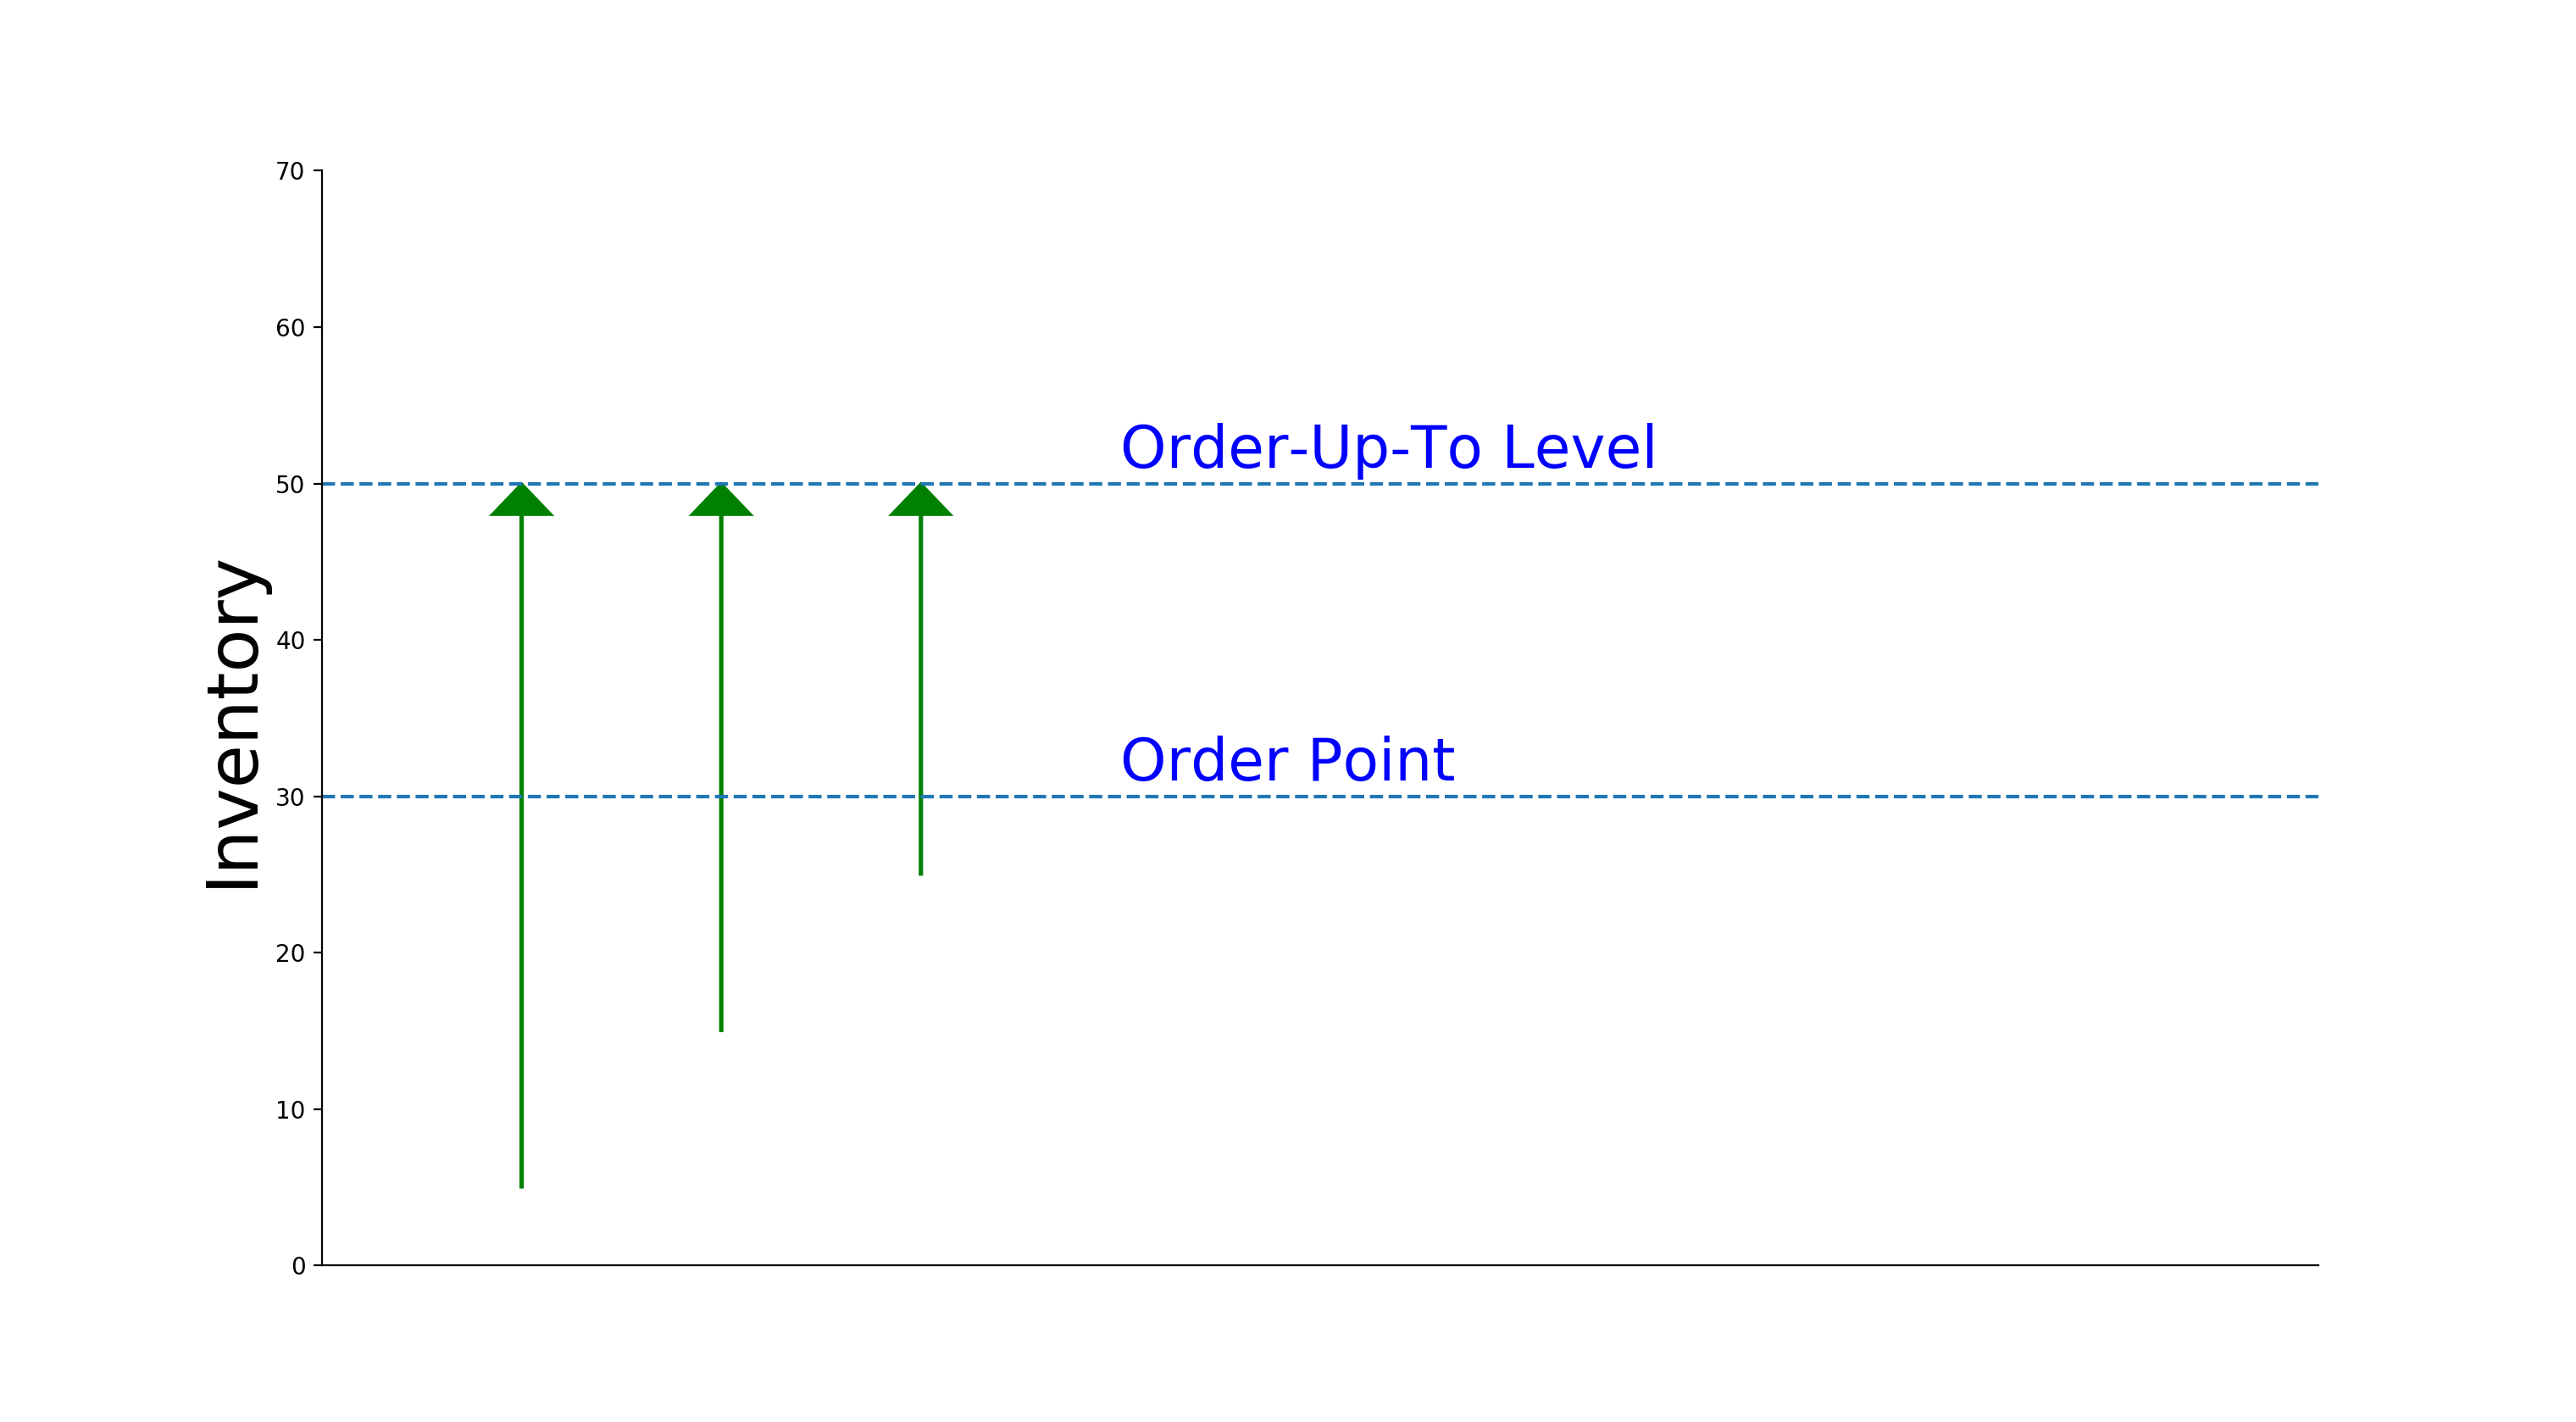
\includegraphics[width=12cm, height=8cm]{op_otl.png}
\end{frame}

\begin{frame}
\frametitle{Costs viewed against End-of-Day Inventory}
\includegraphics[width=12cm, height=8cm]{newsvendor_arrow2.png}
\end{frame}

\begin{frame}
\frametitle{UnderCapacity and OverCapacity Costs}
\includegraphics[width=12cm, height=8cm]{capacity_costs.png}
\end{frame}

\begin{frame}
\frametitle{UnderCapacity Cost: Customer Psychology and Economics}
\pause
\begin{itemize}[<+->]
\item Retail Mantra: ``Stack it high and watch it fly''
\item Customers like to see shelves well stocked
\item Visual emptiness is known to be a sales deterrent
\item So, full-looking shelves are part of presentation strategy
\item At a certain level of emptiness, the deterrent rises sharply
\item Hence the convex nature of this cost curve
\item Note that this curve varies from item to item
\item It also varies from regular season to end of season
\item Modeling/calibrating this is tricky!
\item However, getting a basic model in place is vital
\end{itemize}
\end{frame}

\begin{frame}
\frametitle{OverCapacity Cost: Backroom Space Constraints}
\pause
\begin{itemize}[<+->]
\item Retail store backrooms have limited capacity
\item Typically tens of thousands of items compete for this space
\item Retailers like to have clean and organized backrooms
\item A perfect model is when all your inventory is on store shelves
\item With backroom used purely as a hub for home deliveries
\item Practically, some overflow from shelves is unavoidable
\item Hence, the convex nature of this curve
\item Modeling this is hard because it's a multi-item cost/constraint
\item Again, getting a basic model in place is vital
\end{itemize}
\end{frame}

\begin{frame}
\frametitle{What other costs are involved?}
\pause
\begin{itemize}[<+->]
\item Holding Cost: Interest on Inventory, Superficial Damage, Maintenance
\item Stockout Cost: Lost Sales, sometimes Lost Customers
\item Labor Cost: Replenishment involves movement from truck to shelf
\item Spoilage Cost: Food \& Beverages can have acute perishability
\item End-of-Season/Obsolescence Cost: Intersects with Clearance Pricing 
\end{itemize}
\end{frame}

\begin{frame}
\frametitle{Practical Inventory Control as a Markov Decision Process}
\pause
\begin{itemize}[<+->]
\item The store experiences random daily demand
\item The store can place a replenishment order in casepack mutiples
\item This is an MDP where {\em State} is current Inventory Level at the store
\item {\em State} also includes current in-transit inventory (from warehouse)
\item {\em Action} is the multiple of casepack to order (or not order)
\item {\em Reward} function involves all of the costs we went over earlier
\item State transitions governed by demand probability distribution
\item Solve: Dynamic Programming or Reinforcement Learning Algorithms
\end{itemize}
\end{frame}

\begin{frame}
\frametitle{Inputs to this MDP (other than the costs)}
\pause
\begin{itemize}[<+->]
\item Daily Demand Forecast probability distribution function
\item Shelf Capacity
\item Casepack size
\item Lead Time (time from replenishment order to arrival on shelf)
\end{itemize}
\end{frame}

\begin{frame}
\frametitle{Where do these inputs come from?}
\pause
\begin{itemize}[<+->]
\item From solutions to various other Forecasting and Planning problems
\item Demand Forecasting is a statistical learning problem
\item Planning problems are Optimization problems
\item Some Planning Problems:
\begin{itemize}
\item Assortment Selection
\item Shelf-size Planning
\item Casepack Sizing
\item Network Planning (for Lead Time)
\item Labor Planning
\end{itemize}
\item Some of these planning problems based on Inventory Control solution
\item Chicken-and-egg issues resolvable by Simulations
\item Very important to design the interfaces consistently
\item Clean software framework for overall system design is vital to success
\end{itemize}
\end{frame}

\begin{frame}
\frametitle{Calibrating the Cost Parameters}
\begin{itemize}
\item slide under construction ...
\end{itemize}
\end{frame}

\begin{frame}
\frametitle{Combining Price Control with Inventory Control}
\pause
\begin{itemize}[<+->]
\item Clearance Pricing: Optimizing price markdowns at end-of-season
\item So as to maximize your total profit (sales revenue minus costs)
\item Note: There is a non-trivial cost of performing a markdown
\item If markdowns are small, we end up with surplus at season-end
\item Surplus often needs to be disposed at poor salvage price
\item If markdowns are large, we run out of Christmas trees early
\item Sometimes, stockout cost at end-of-season can be very high
\item {\em State} is [Days Left, Current Inventory, Current Price, Market Info]
\item {\em Action} is Price Markdown
\item {\em Reward} includes Sales revenue, markdown cost, stockout cost, salvage
\item {\em Reward} \& {\em State}-transitions governed by {\em Price Elasticity of Demand}
\item Ambitious: Joint MDP with {\em Action} as Replenishment \& Markdown

\end{itemize}
\end{frame}



\end{document}
